% !TEX root = ../Thesis.tex

\chapter{Utilizzo dei progetti in un server reale}
\label{cap:capitolo4}
Per fornire un esempio di utilizzo dei progetti presentati nei capitoli precedenti, si è deciso di installare OpenNebula su un computer di prova. Il computer scelto è un desktop posizionato all'interno di una stanza ad uso degli studenti di informatica. Il computer non è raggiungibile dall'esterno ma è accessibile tramite rete cablata e wifi interna alla stanza. Questo permette di avere un ambiente di test semplice ma vicino alla realtà.\par
Le specifiche principali del desktop sono:
\begin{itemize}
    \item processore: Intel Core i7-13700 (24 core);
    \item scheda grafica integrata: Intel UHD 770;
    \item RAM: 32 GB ddr5.
\end{itemize}
Questo computer servirà sia come gestore degli host che come uno degli host stessi. L'operazione è tranquillamente consentita in OpenNebula; da ora in avanti questo computer sarà riferito come \emph{server}.
In questo esempio è stato considerato anche un altro host, un computer portatile presente nella stessa rete del \emph{server} OpenNebula con le seguenti specifiche:
\begin{itemize}
    \item processore: Intel Core i5-8350U (8 core);
    \item scheda grafica integrata: Intel UHD 620;
    \item RAM: 8 GB ddr4.
\end{itemize}
Questo computer sarà riferito da qui in avanti come \emph{laptop}.\par
Le policy scelte sono state quelle per il load balancing. Questa scelta è data dal fatto che il \emph{server} è molto più potente del \emph{laptop} e quindi sarà facile vedere se il bilanciamento viene fatto correttamente.

\section{Installazione dei due progetti}
In questo capitolo non sarà presa in considerazione l'installazione di OpenNebula; tutte le procedure descritte in questa sezione saranno riferite ad un sistema in cui OpenNebula è già installato e funzionante (per informazioni sulle procedure seguite fare riferimento alla ducumentazione ufficiale\footnote{\url{https://docs.opennebula.io/6.8/installation\_and\_configuration/frontend\_installation/install.html}}). Stessa considerazione è fatta anche per i nodi\footnote{\url{https://docs.opennebula.io/6.8/open\_cluster\_deployment/kvm\_node/kvm\_node\_installation.html}}.\par
Per eseguire correttamente il codice descritto nel capitolo \ref{cap:capitolo3} è stato necessario innanzitutto aprire un terminale ad autenticarsi come utente del gruppo \emph{oneadmin}, da cui si è dovuto clonare la repository github per poi seguire le procedure descritte nel file \texttt{README.md}. Si evidenzia come sia fondamentale che l'utente che esegue i comandi sul terminale da qui in avanti abbia diritti di lettura, scrittura e esecuzione sui file appropriati, di conseguenza è consigliato direttamente clonare la repository con l'utente corretto; i permessi si possono fornire in un secondo momento se lo si preferisce, ma se non risultano del tutto corretti i risultati potrebbero essere inaspettati.
In questo caso si vuole testare il funzionamento di \emph{policy\_manager} di conseguenza i passaggi da seguire sono:
\begin{itemize}
    \item Lato \emph{server}:
\begin{itemize}
    \item entrare nella cartella \emph{resource\_management} ed eseguire il comando \texttt{mvn install} assicurandosi che tutti i test che sono eseguiti abbiano successo. Questo comando installerà il progetto all'interno della repository locale di Maven, passaggio fondamentale per eseguire con successo il comando successivo;
    \item entrare nella cartella \emph{policy\_manager} ed eseguire il comando \texttt{mvn test} per assicurarsi che i test vadano a buon fine e tutto possa funzionare correttamente;
    \item ancora all'interno della cartella \emph{policy\_manager} eseguire il comando \texttt{mvn spring-boot:run} per far partire il server gestito con Spring-Boot.
    \item entrare nella cartella \emph{policy\_manager/config.properties} e modificare i campi in modo consono con la propria installazione di OpenNebula. In questo caso abbiamo considerato i due host di \emph{ID} 0 e 2, e i due template di \emph{ID} 0 e 1. Il file di configurazione avrà quindi la seguente forma:
    \begin{lstlisting}[xleftmargin=1em, label={code:config_properties}, caption={config.properties}]
hyper1.host.id=0
hyper2.host.id=2
type1.template.id=0
type2.template.id=1
context.file.location=opennebula_context_actions/
    \end{lstlisting}
\end{itemize}
    \item lato client \emph{da eseguire una volta}:
    \begin{itemize}
        \item connettersi all'ip del server sulla porta 8080;
        \item validare le policy che si vogliono utilizzare, in questo caso abbiamo scelto quelle di load balancing presenti nel progetto;
        \item modificare le policy per aderire al caso reale in questione. In particolare quindi inserire i corretti \emph{ID} degli host e dei template. Ovviamente questo passaggio può essere saltato se si scrivono le policy direttamente per il proprio sistema senza usarne di generiche già scritte;
    \end{itemize}
    \item lato client \emph{da eseguire ogni volta}:
    \begin{itemize}
        \item connettersi all'ip del server sulla porta 8080;
        \item creare una richiesta con il menù a tendina disponibile e validarla;
        \item inviare la richiesta;
    \end{itemize}
\end{itemize}
Nel nostro esempio di test tutti i passaggi hanno funzionato senza alcun problema, anche se in una precedente installazione su un altro server si era evidenziata la necessità di inserire alcune dipendenze nel file \texttt{pom.xml} rispetto a quelle che erano necessarie sul computer di test originale. Si evidenzia inoltre come non sia stato necessario modificare alcun file .java.

\section{Specifiche dell'esempio}
Le valutazioni fatte da FACPL sono visibili direttamente nel terminale da cui è stato eseguito il comando \texttt{mvn spring-boot\:run}. Le informazioni sull'applicazione delle policy e l'invio delle richieste, oltre che le informazioni sulle azioni svolte sulle virtual machine, sono visibili nei file di log posti nella cartella \emph{logs}.\par
L'utente può connettersi a OpenNebula Sunstone, accessibile di default sulla porta 9869 del server per vedere la situazione delle virtual machine e degli host. Per farlo deve però essere in possesso delle credenziali di un account di OpenNebula.\par
Nel nostro caso di esempio abbiamo considerato degli utenti che si connettono alla web-app di \emph{policy\_manager} attraverso la rete wifi. Nessun utente ha la possibilità di modificare le policy, però tutti possono vederle e quindi formattare le loro richieste di conseguenza. Alcuni utenti appartengono al gruppo P\_2 mentre altri al gruppo P\_1, quindi è possibile verificare il cambiamento del sistema all'invio di specifiche richieste da entrambi i gruppi.

\section{Risultati dell'esecuzione}
Di seguito sono riportate le prime richieste e i risultati del loro invio sulla dashboard di OpenNebula:
\begin{figure}[H]
    \centering
    \begin{minipage}{1\textwidth}
        \centering
        
\includegraphics[width=\textwidth]{tesi_screenshot/OpenNebula_firstVM.png}
        \caption{Dashboard di OpenNebula con una sola virtual machine}
    \end{minipage}
    \begin{minipage}{0.49\textwidth}
        \centering
        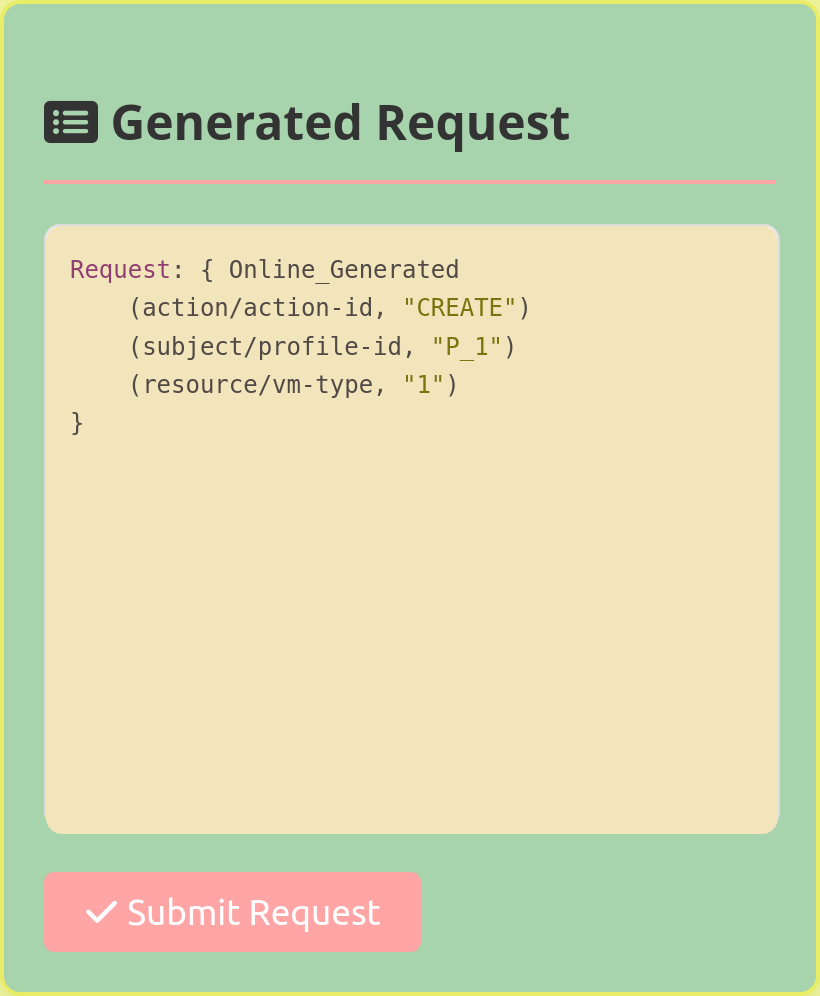
\includegraphics[width=\textwidth]{tesi_screenshot/P1Create_1.png}
    \end{minipage}
    \begin{minipage}{0.49\textwidth}
        \centering
        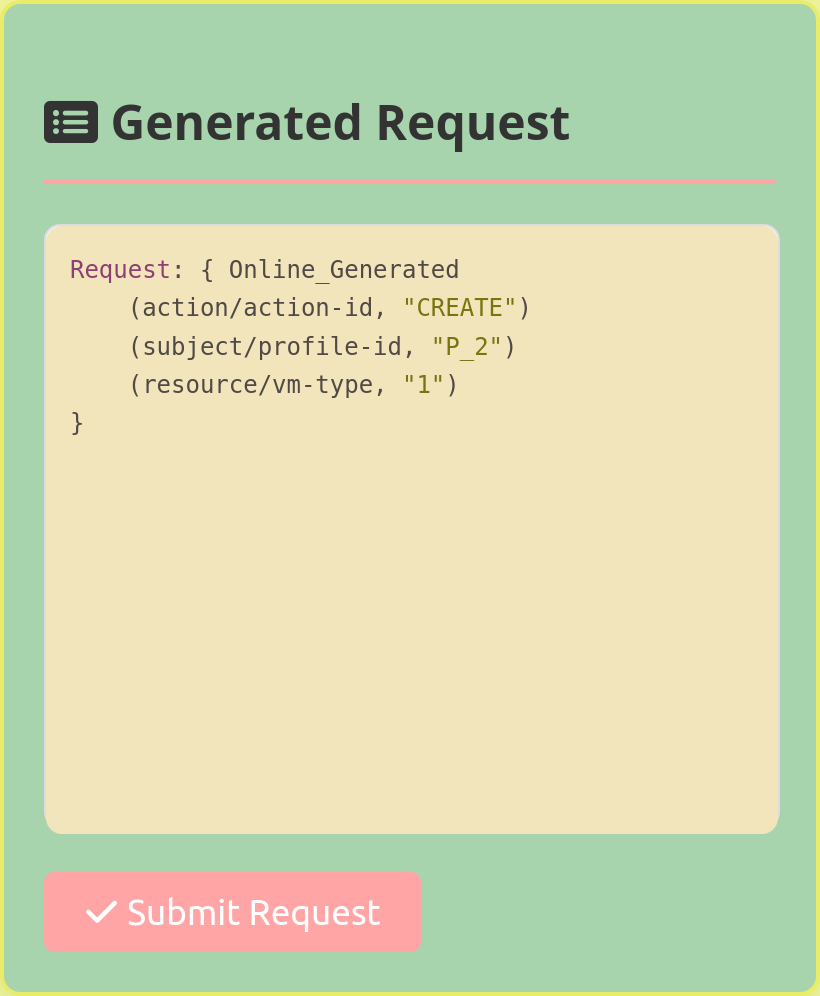
\includegraphics[width=\textwidth]{tesi_screenshot/P2Create_1.png}
    \end{minipage}
    \caption{Richieste di P\_1 e P\_2}
\end{figure}
Come si può vedere nonostante siano state eseguite due richieste è stata creata soltanto una macchina virtuale. Questa logica è corretta perchè l'utente P\_1 non è autorizzato a creare virtual machine con il template 1. Le valutazione del sistema FACPL sono quindi:
\begin{figure}[H]
    \begin{minipage}{0.27\textwidth}
        \centering
        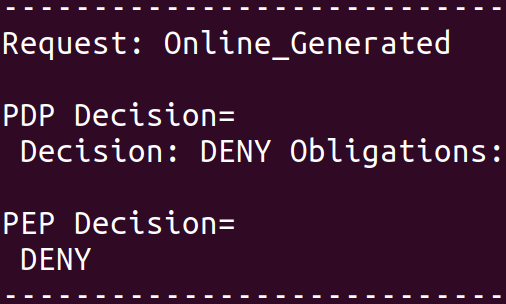
\includegraphics[width=\textwidth]{tesi_screenshot/DenyP1_1_cut.png}
    \end{minipage}
    \begin{minipage}{0.72\textwidth}
        \centering
        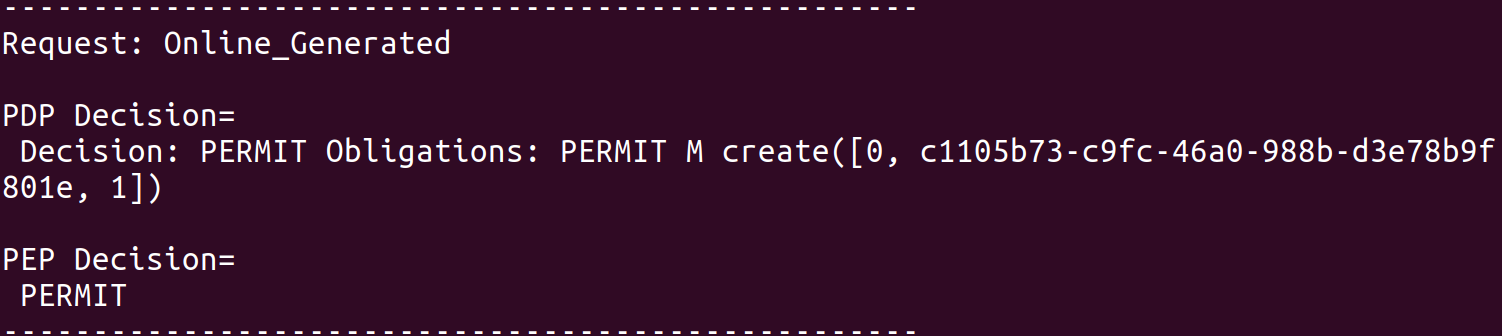
\includegraphics[width=\textwidth]{tesi_screenshot/Permit_P2_1.png}
    \end{minipage}
    \caption{Valutazioni di FACPL sulle due richieste}
\end{figure}
A questo punto sono state inviate ulteriori richieste da utenti con \emph{ID} P\_2 sia per virtual machine di tipo 1 che per virtual machine di tipo 0. Si nota che il sistema continua ad inserire tutte le virtual machine sul \emph{server} fino a che non si raggiunge un bilanciamento di risorse rimaste tra \emph{server} e \emph{laptop}:
\begin{figure}[H]
    \centering
    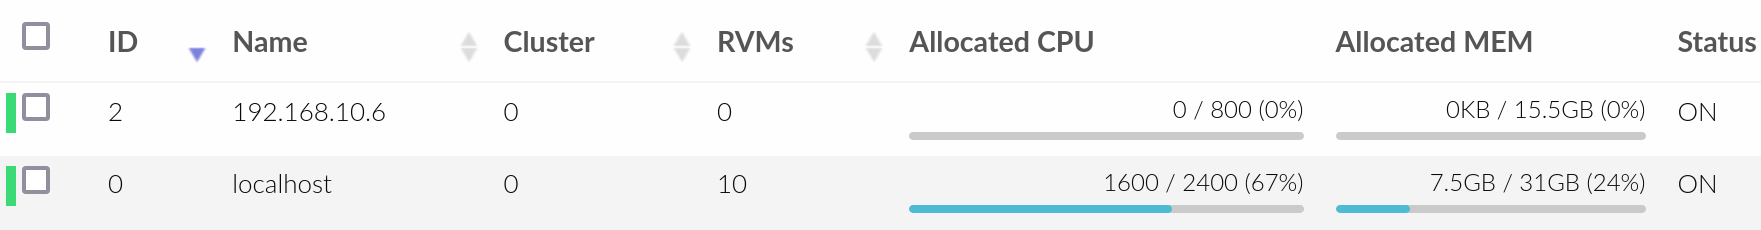
\includegraphics[width=\textwidth]{tesi_screenshot/OpenNebula_eavenLoad.png}
    \caption{Dashboard di OpenNebula con i due host bilanciati}
\end{figure}
Il load balancing sembra quindi funzionare correttamente. Per mostrarlo ulteriormente si continuano a creare delle virtual machine di modo da verificare che comincino ad essere aggiunte anche all'interno del \emph{laptop}:
\begin{figure}[H]
    \centering
    \includegraphics[width=\textwidth]{tesi_screenshot/alternating.png}
    \caption{Dashboard con le virtual machine alternate fra i due host}
\end{figure}
Continuando in questo modo si raggiunge una situazione in cui entrambi gli host hanno tutte le CPU utilizzate al 100\%. A questo punto secondo le policy scelte il sistema dovrebbe controllare se ci sono alcune virtual machine di tipo 1 da freezzare in favore della creazione di virtual machine di tipo 2. Questo infatti è quello che succede:
\begin{figure}[H]
    \centering
    \begin{minipage}{\textwidth}
        \centering
        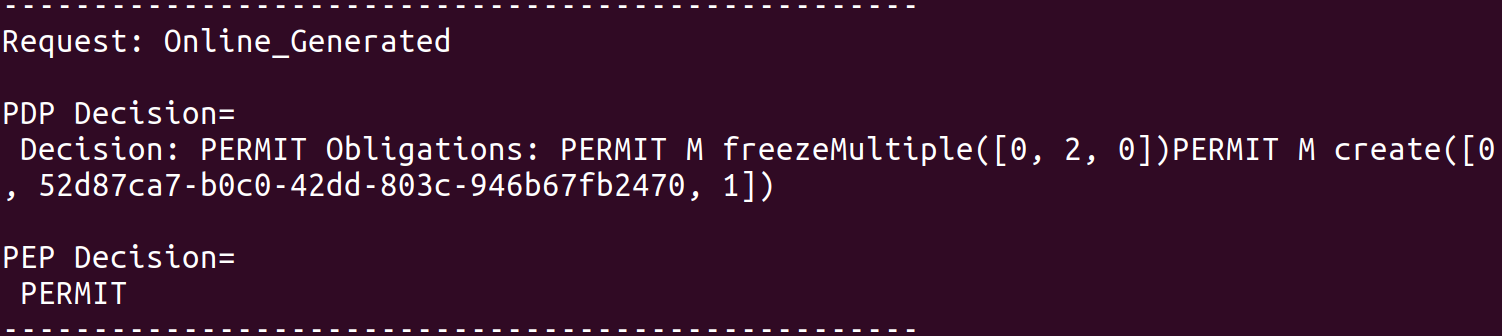
\includegraphics[width=\textwidth]{tesi_screenshot/permitReleaseCreateLonger.png}
        \caption{Valutazione di FACPL}
        \label{fig:full_hosts}
    \end{minipage}
    \begin{minipage}{\textwidth}
        \centering
        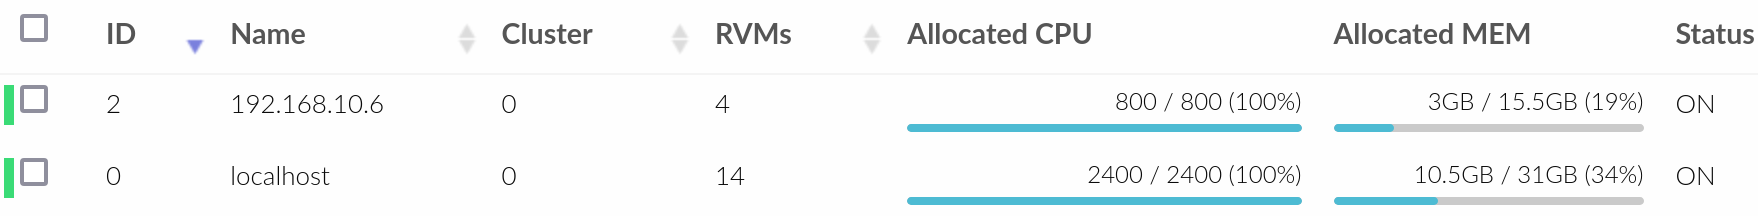
\includegraphics[width=\textwidth]{tesi_screenshot/full_hosts.png}
        \caption{Dashboard con entrambi gli host al 100\% di utilizzo}
        \label{fig:full_hosts}
    \end{minipage}
    \par \medskip
    \begin{minipage}{\textwidth}
        \centering
        
\includegraphics[width=\textwidth]{tesi_screenshot/stoppedVMS.png}
        \caption{virtual machine stoppate automaticamente}
    \end{minipage}
\end{figure}
Le due virtual machine freezzate erano appartenenti al \emph{server}, anche perchè era l'unico dei due host ad avere macchine di tipo 1 attive e quindi freezzabili. Possiamo notare questo anche nella figura \ref{fig:full_hosts}, dato che il numero delle virtual machine sul \emph{server} è 14. Questo numero è dato dalla presenza di 10 virtual machine che richiedono 2 processori l'una e 4 virtual machine che richiedono 1 processore l'una. Sul \emph{laptop} ci sono invece soltanto 4 virtual machine che richiedono 2 processori l'una.\par
Se si tenta di creare ulteriori virtual machine di tipo 1 il sistema FACPL ritorna correttamente una valutazione di \emph{DENY} e quindi la richiesta non viene neanche inviata a OpenNebula come si può vedere nella seguente immagine:
\begin{figure}[H]
    \centering
    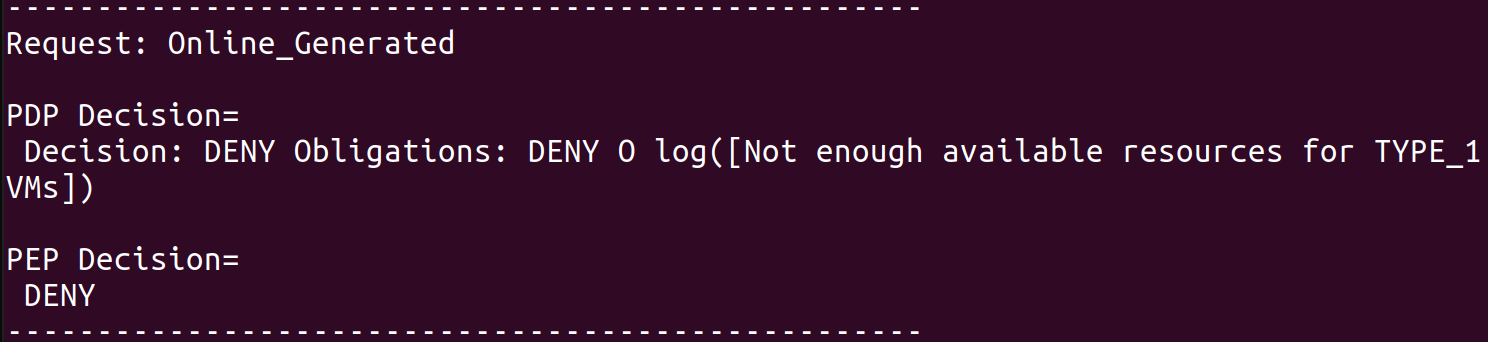
\includegraphics[width=\textwidth]{tesi_screenshot/notEnoughResources.png}
\end{figure}
Questo è un comportamento corretto dato che in realtà OpenNebula permette di sovraccaricare il sistema ma non è quello che vogliamo nel nostro caso.\par

A questo punto l'unico passo rimasto è testare se le macchine vengono correttamente rilasciate anche con l'utilizzo diretto delle richieste di tipo \emph{RELEASE}. Per fare questo si è resettato il sistema, si è poi creato una virtual machine e si è verificato che FACPL valutasse correttamente la richiesta di rilascio della stessa. Come si può vedere nelle seguenti figure l'esecuzione è andata a buon fine:
\begin{figure}[H]
    \centering
    \begin{minipage}{.5\textwidth}
        \centering
        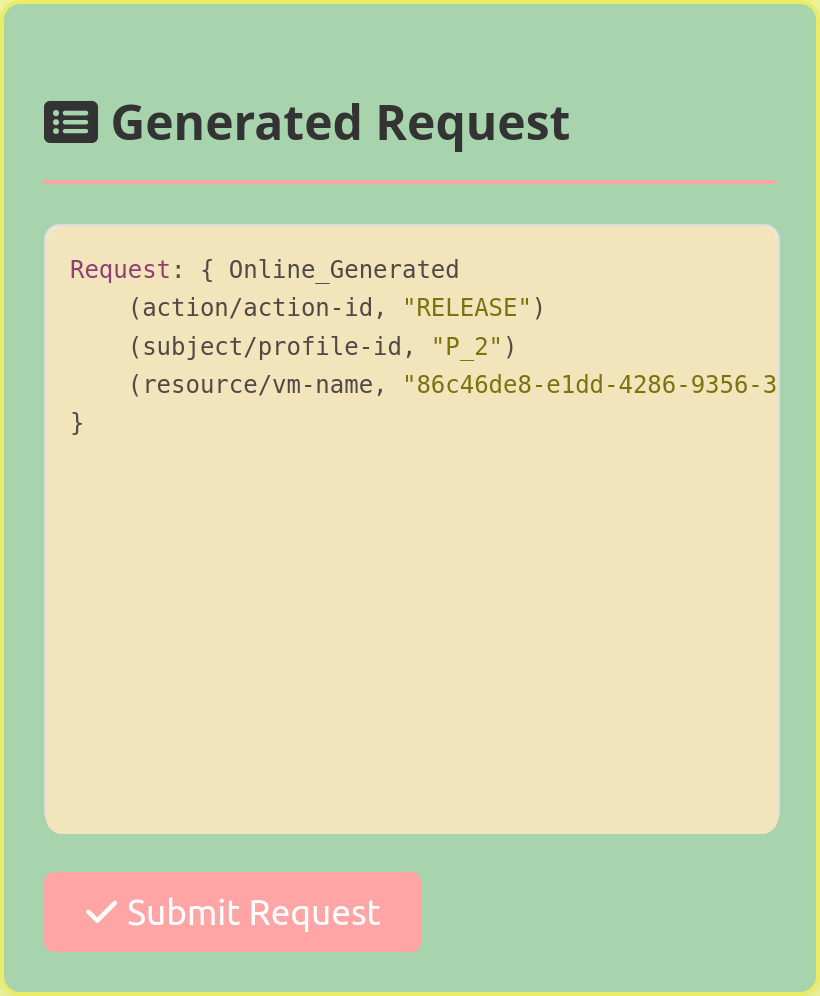
\includegraphics[width=\textwidth]{tesi_screenshot/ReleaseP2.png}
        \caption{Richiesta di rilascio}
    \end{minipage}
    \begin{minipage}{\textwidth}
        \centering
        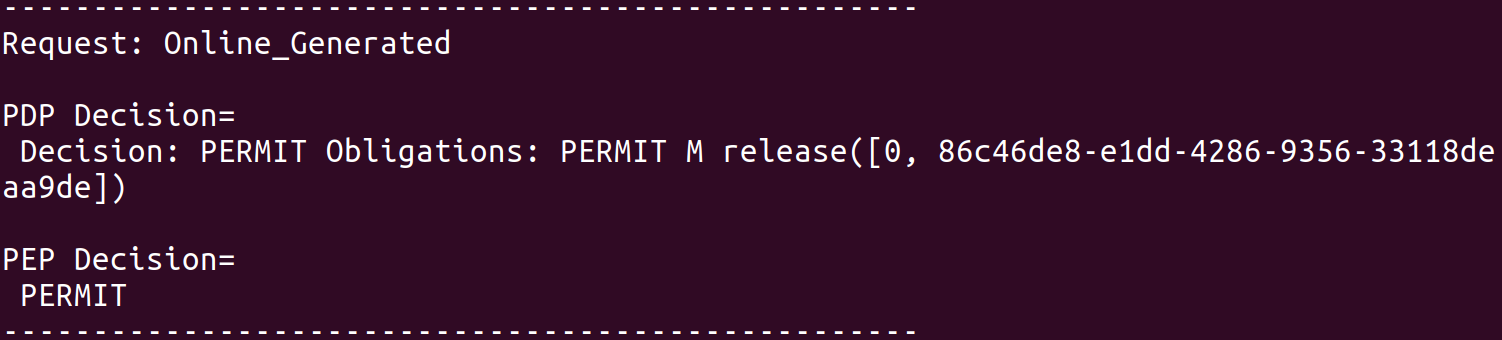
\includegraphics[width=\textwidth]{tesi_screenshot/permitRelease.png}
        \caption{valutazione di FACPL}
    \end{minipage}
    \par \medbreak
    \begin{minipage}{\textwidth}
        \centering
        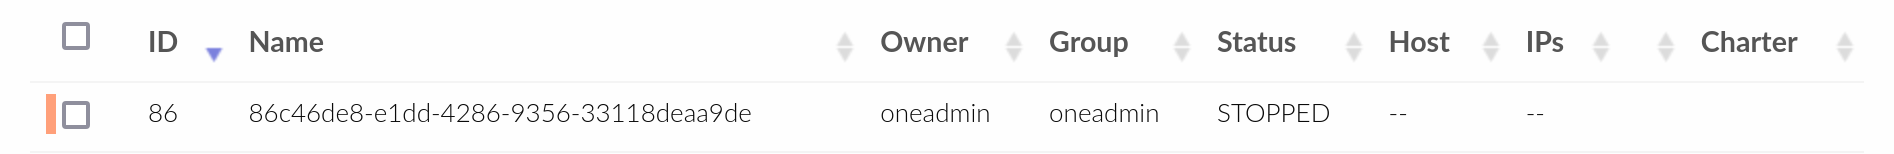
\includegraphics[width=\textwidth]{tesi_screenshot/stoppedVM.png}
        \caption{Virtual machine stoppata}
    \end{minipage}
\end{figure}